\documentclass{article}
\usepackage[utf8]{inputenc}
\usepackage{hyperref}
\usepackage{amsmath}
\usepackage{amsfonts}
\usepackage{graphicx}


\title{SPhO Ten Year Series (TYS) with Solutions: 2016 Questions}
\author{
    Solutions available on Victoris\\
    \texttt{victoris.org}
    % new collaborators add your name and contact here!
}

\date{\today}

\begin{document}
\maketitle

\section{2016}

\subsection{Question 1}
1. Hohmann transfer orbit and gravity assist

(a) A spacecraft is to be sent from Earth to Saturn. The Hohmann transfer is a manoeuvre that transfers the
spacecraft from Earth’s orbit around the Sun (assumed to be circular) to Saturn’s orbit around the Sun (assumed
to be circular also). This is done by pushing the spacescraft into an elliptical orbit that has its perihelion and
aphelion touching Earth’s orbit and Saturn’s orbit, respectively.

\begin{figure}
	\centering
	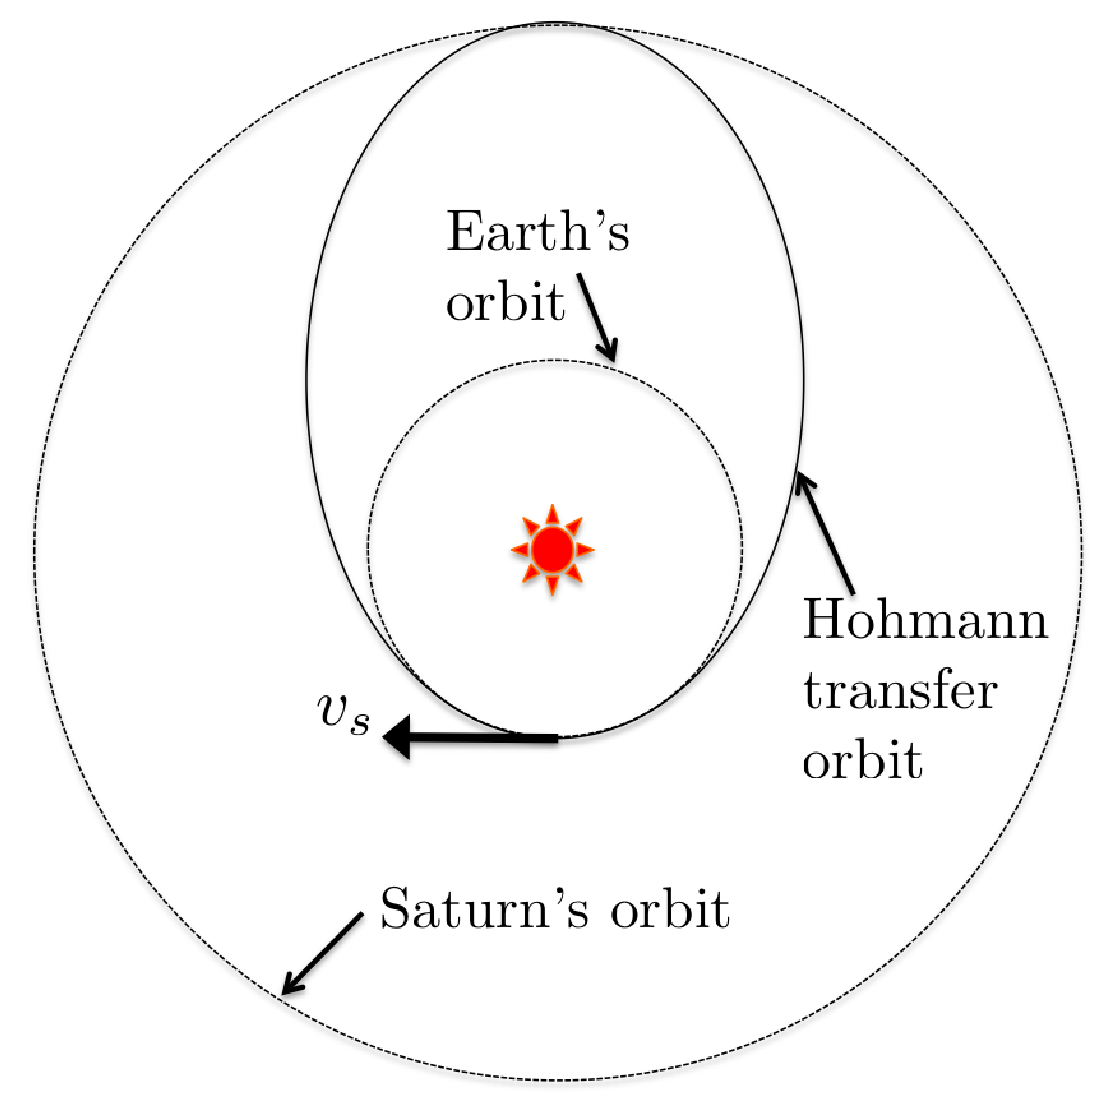
\includegraphics[width=0.5\linewidth]{spho_book_TYS_images/2016q1.png}
	\caption{Hohmann transfer orbit from Earth to Saturn. $v_s$, is the velocity of the spacecraft.}
\end{figure}

(i) Assuming that the spacecraft is initially travelling at the velocity of Earth around the Sun, calculate the change in velocity $\Delta v$ for the spacescraft to transfer from Earth's orbit to the elliptical orbit. Ignore the Earth's and Saturn's gravitational forces on the spacecraft. Use the constants below (and their corresponding symbols) in your working. [4 marks] \\
Earth's velocity around Sun: $v_{\oplus}=2.97 \times 10^{4} \mathrm{~m} / \mathrm{s}$ \\
Earth's orbital radius $r_{\oplus}=1.50 \times 10^{11} \mathrm{~m}$ \\
Saturn's orbital radius $r_{h}=1.43 \times 10^{12} \mathrm{~m}$ \\
Mass of Sun $M_{\odot}=1.99 \times 10^{30} \mathrm{~kg}$ \\
Gravitational constant $G=6.67 \times 10^{-11} \mathrm{Nm}^{2} / \mathrm{kg}^{2}$ \\
(ii) Calculate the time it takes for the spacecraft to travel from Earth's orbit to Saturn's orbit. [2 marks] \\
(b) The Cassini spacecraft was not sent to Saturn by a direct Hohmann transfer. Instead, it was first sent to Venus (via Hohmann transfer), where it gained speed, twice, using gravity assists by Venus. The first gravity assist by Venus changed the spacecraft's velocity and transferred the spacecraft to a more eccentric orbit, such that the spacecraft returned to its orbital perihelion after Venus had completed its orbit twice, and the spacecraft received the second gravity assist by Venus at that point. Calculate the change in velocity of the spacecraft during the first Venus' gravity assist. [6 marks]\\
Venus' orbital radius $r_{v}=1.08 \times 10^{11} \mathrm{~m}$ \\
Venus' orbital period $T_{v}=0.615$ years \\

\subsection{Question 2}
2. Consider a rigid axially symmetric wheel with mass $M$, moment of inertia $I$ about the axis of symmetry $S$, and radius $R$, moving in an upright position on a horizontal plane. The coefficient of kinetic friction between the wheel and the plane is $\mu_{k}$ \\
(a) The wheel is initially spun about $S$ with constant angular speed $\omega_{0}$, and is then released. It slips for a time $T_{a}$ and then rolls without slipping. Determine $T_{a}$ and the centre-of-mass speed $v_{a}$ of the rolling wheel. [4 marks] \\ 

\begin{figure}
	\centering
	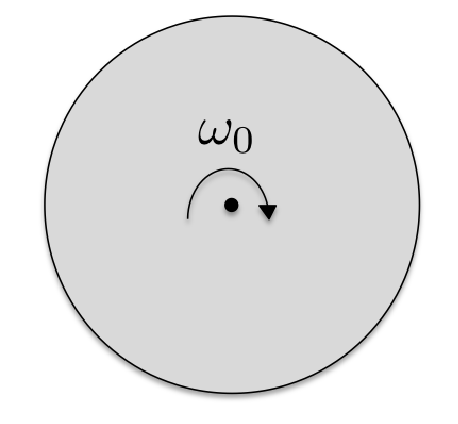
\includegraphics[width=0.5\linewidth]{spho_book_TYS_images/2016q2.png}
	\caption{Rolling wheel with initial angular speed $\omega_0$.}
\end{figure}

(b) The wheel has an initial horizontal centre-of-mass speed $v_{0}$ in addition to an initial angular speed $\omega_{0}$. Determine the time $T_{b}$ at which the wheel rolls without slipping and the centre of mass speed $v_{b}$ of the rolling wheel. [4 marks] 
\begin{figure}
	\centering
	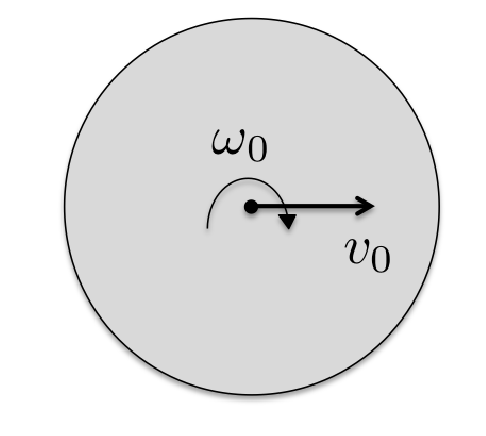
\includegraphics[width=0.5\linewidth]{spho_book_TYS_images/2016q2_2.png}
	\caption{Rolling wheel with initial angular speed $\omega_{0}$ and initial horizontal centre-of-mass speed $v_{0}$.}
\end{figure}

(c) The wheel has an initial horizontal centre of mass speed $v_{0}$ and an initial backspin $-\omega_{0}$. Determine the possible motions of the wheel. [4 marks]
\begin{figure}
	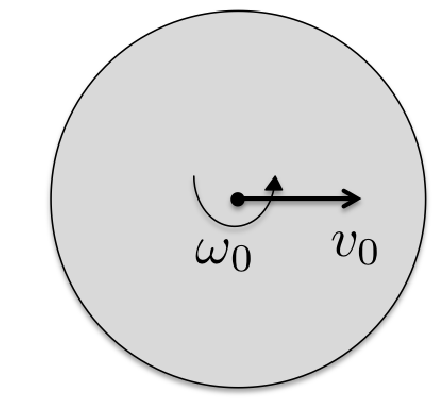
\includegraphics[width=0.5\linewidth]{spho_book_TYS_images/2016q2_3.png}
	\caption{Rolling wheel with initial backspin of angular speed $\omega_{0}$ and initial horizontal centre-of-mass speed $v_{0}$.}
\end{figure}

\subsection{Question 3}
3. A circular coil with radius $a$ is connected with an equilateral triangle on the inside as shown in the figure below. The resistance for each section of the wire is labeled. A uniform magnetic field $B(t)$ is pointing into the paper, perpendicular to the plane of the coil. $B(t)$ is decreasing over time at a constant rate $k .$ Given $2 r_{1}=3 r_{2} .$ Find $U_{A B}$, the potential difference between points $\mathrm{A}$ and $\mathrm{B}$. [10 marks]
\begin{figure}
	\centering
	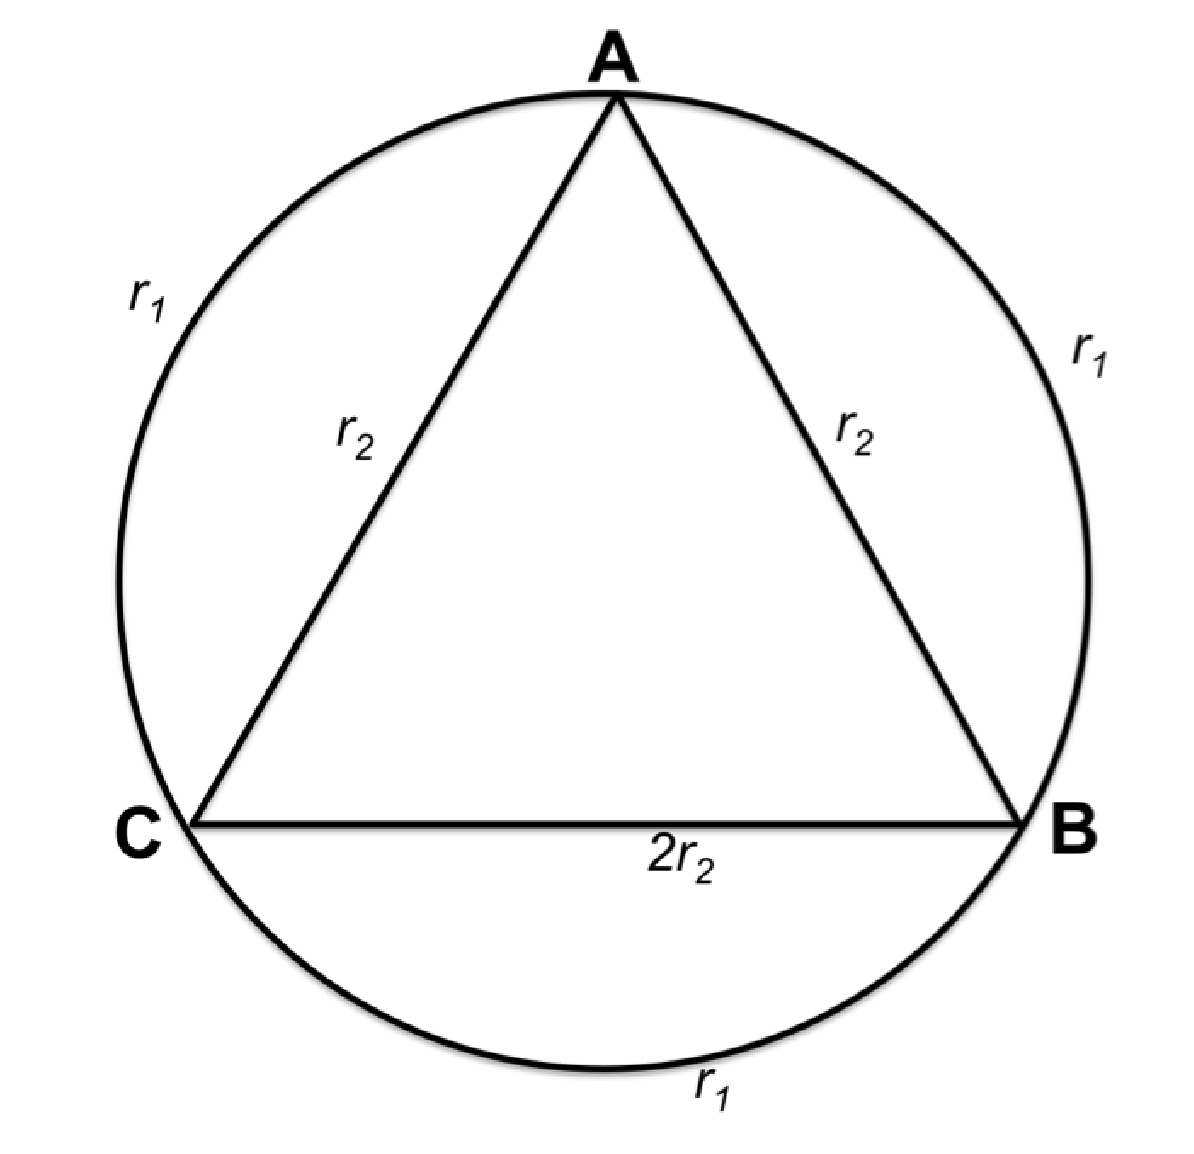
\includegraphics[width=0.5\linewidth]{spho_book_TYS_images/2016q3.png}
	\caption{Circular coil with 3 wires forming an equilateral triangle inside the circle.}
\end{figure}

\subsection{Question 4}
4. An experiment was performed to determine the value of the gravitational acceleration $g$ on Earth. Two equal masses of mass $M$ hang at rest from the ends of a string on each side of a light pulley (see figure below). A mass $m=0.01 M$ is placed on the right-hand-side mass. After the heavier side has moved down from rest by $h=1 \mathrm{~m}$ the small mass $m$ is removed. The system continues to move for the next $1 \mathrm{~s}$, covering a distance of $H=0.312 \mathrm{~m} .$ Find the value of $g$. [10 marks]
\begin{figure}
	\centering
	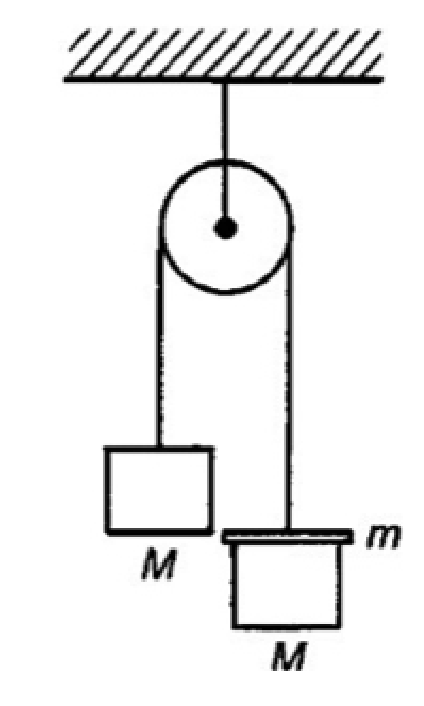
\includegraphics[width=0.5\linewidth]{spho_book_TYS_images/2016q4.png}
	\caption{Pulley with a system of masses attached.}
\end{figure}

\subsection{Question 5}
5. Consider the following decay
$$
{ }^{228} \mathrm{Th} \rightarrow{ }^{224} \mathrm{Ra}+\alpha
$$
The available energy $Q$ is given by
$$
Q=\left(m_{\mathrm{Th}}-m_{\mathrm{Ra}}-m_{\alpha}\right) c^{2}
$$
where $m_{\mathrm{Th}}, m_{\mathrm{Ra}}$, and $m_{\alpha}$ are the masses of Th-228, Ra-224 and the alpha particle respectively. \\
(a) Calculate the percentage of $Q$ carried by the alpha particle. [6 marks] \\
(b) In the above decay, the highest energy $\alpha$ particle has energy $5.423 \mathrm{~MeV}$ and the next highest energy is $5.341$ $\mathrm{MeV}$. Find the energy of the first excited state of Ra-224. [3 marks]

\subsection{Question 6}
6. We know that a rainbow can be formed by a ray entering a water droplet and exiting it after suffering a total internal reflection. We can call this a 'first-order' rainbow. The question is regarding the possibility of a 'zeroth' order rainbow where parallel rays impinging on a spherical raindrop is refracted into the drop and then out again into the air directly (without total internal reflection). \\
(a) Sketch a diagram depicting such a situation in a raindrop. Find the angle of deviation in terms of the angle of incidence $\theta_{i}$ and angle of refraction $\theta_{r}$. [2 marks] \\
(b) Show that the 'zeroth' order rainbow, given the above conditions, cannot exist. [3 marks] \\
In the following part of the question, we ask if a rainbow (or 'bubblebow') is able to be formed from the scattering of light in air bubbles in water. Again, we can consider parallel rays (i) entering the bubble and exiting without total internal reflection and (ii) entering and exiting with one (assumed) internal reflection at the gas-liquid interface. [3 marks] \\
(c) Sketch a diagram/s depicting the two situations in the bubble. Find the angle of deviation in each case. [3 marks]\\
(d) Work out if a rainbow (or 'bubblebow') can exist in each case. [4 marks] 

\subsection{Question 7}
7. Two infinitely long concentric hollow cylinders have radii $a$ and $4 a$. Both cylinders are insulators; the inner cylinder has a uniformly distributed charge per length of $+\lambda$; the outer cylinder has a uniformly distributed charge per length of $-\lambda$. \\
The inner cylinder is rotating clockwise about its axis with an angular velocity $\omega \ll c / a$, where $c$ is the speed of light. Assume that the permeability of the dielectric cylinder and the space between the cylinders is that of free space, $\mu_{0}$. \\
(a) Determine the electric field for all regions. [4 marks] \\
(b) Determine the magnetic field for all regions [4 marks] \\
(c) Determine the Poynting vector $\mathbf{S}=\frac{1}{\mu_{0}} \mathbf{E} \times \mathbf{B}$, for all regions. [2 marks]

\subsection{Question 8}
8. Consider a spaceship initially at rest in the lab frame. At a given instant, it starts to accelerate with constant proper acceleration $a$. Assume that the lab clock $(t)$ and spaceship clock $\left(t'\right)$ are synchronized such that this happens when $t=t'=0$. [Note: Proper acceleration is defined such that: at t'+dt', the spaceship is moving at speed a dt' relative to the frame it was in at time t'.] \\
(a) Determine the relative speed of the spaceship and the lab frame in terms of $t'$. Also, check the limit of the relative speed found when $a t' \ll c$ and comment. [5 marks] \\
(b) Find the relation between $t$ and $t'$ at later stage. Also, explore the relation for condition $a t' \gg c$. Comment. [5 marks] \\

\subsection{Question 9}
9. An electron bubble in liquid helium (adapted from APhO 2010 Taipei) \\
When an electron is planted inside liquid helium, it can repel the atoms around it isotropically, thus forming a spherical surface, inside which contains nothing but the electron itself. This is known as an electron bubble. \\
\\
The components of an electron's position vector $\vec{q}=(x, y, z)$ and momentum vector $\vec{p}=\left(p_{x}, p_{y}, p_{z}\right)$ must obey Heisenberg's uncertainty relations $\Delta q_{i} \Delta p_{i} \geq h / 4 \pi$, where $h$ is the Planck constant. \\
Note that the uncertainty of a variable $f$, denoted by $\Delta f$ is given by
$$
\Delta f=\sqrt{\overline{f^{2}}-\bar{f}^{2}}
$$
where the overhead bar denotes the average (mean) of the quantity under it. \\
Consider an electron bubble in liquid helium with an equilibrium radius $R$. The electron of mass $m$ moves freely inside the bubble with kinetic energy $E_{K}$ and exerts a pressure $P_{e}$ on the inner side of the bubble-liquid interface. The pressure exerted by liquid helium on the outer side of the interface is $P_{\text {He }}$. The liquid is kept at a constant temperature close to $0 \mathrm{~K}$ and the surface tension $\sigma$ is given by $3.75 \times 10^{-4} \mathrm{Nm}^{-1}$.  \\
(a) Find a relation between $P_{\mathrm{He}}, P_{e}$ and $\sigma$. [2 marks] \\
(b) Find a relation between $E_{K}$ and $P_{e}$. [4 marks] \\
(c) Let $E_{0}$ be the smallest possible value of $E_{K}$ consistent with Heisenberg's uncertainty relations when the electron is inside the bubble of radius $R$. Estimate $E_{0}$ as a function of $R$. [4 marks] \\
(d) Let $R_{e}$ be the equilibrium radius of the bubble when $E_{K}=E_{0}$ and $P_{\mathrm{He}}=0 .$ Obtain an expression for $R_{e}$ and calculate its value. [2 marks]


\end{document}
